\section{Kernel}

\begin{frame}{ \textit{Kernel} de GNU Linux}
 \begin{itemize}
  \item 2,4 millones de lineas de código(y contando...)
  \item El 70\% del código son drivers
  \item Windows: mas del doble de lineas!
  \item Tasa de errores en drivers con respecto al Kernel: 7 veces mas
  	\begin{itemize}
 	  \item Fuente:http://pdos.csail.mit.edu/6.097/readings/osbugs.pdf 
  	\end{itemize}
    \item Comparación con la aeronaútica: 
 	\begin{itemize}
   	\item Aislamiento de fallas
	\item Un problema en el toilet no afecta al sistema de navegación!  
  	\end{itemize}
 \end{itemize}	

\end{frame}


\begin{frame}{Kernel Monolítico - Mismo proceso}
  \begin{center}
    \fbox{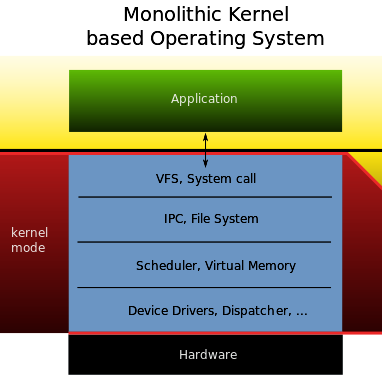
\includegraphics[width=0.4\textwidth]{images/kernel-mono.png}}
   \end{center}
 \begin{itemize}
    \item Todos los componentes del kernel linkeados en un mismo binario en memoria.
    \item Memoria Compartida(sincronización!) 
    \item Scheduler, Drivers, Memory Manager,etc en un mismo proceso 
   \end{itemize} 
\end{frame}

\begin{frame}{Kernel Monolítico - Operating System Crash}

 \begin{itemize}
    \item ¿Que sucede si hay un error en un driver?
    \begin{itemize}
    	\item Windows: BSD(blue screen of death).
    	\item Unix: Kernel Panic.
    \end{itemize}
    \item Un único gran componente linkeado en un mismo espacio de direcciones implica un módulo muy grande y complejo.
    \item La razón de tener un único gran componente linkeado en un mismo espacio de direcciones se debe a cuestiones de performance por limitaciones de hardware tomadas hace mucho tiempo.
     \item ¿Hoy en dia la decisión seria la misma? 
   \end{itemize} 
\end{frame}


\begin{frame}{Microkernel - Procesos de usuario}
  \begin{center}
    \fbox{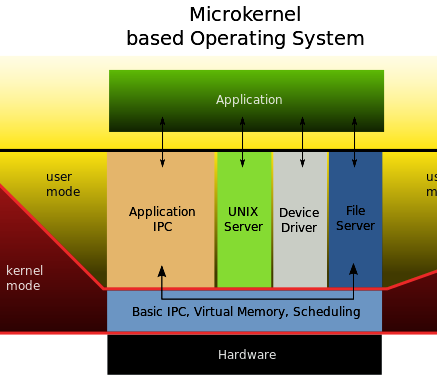
\includegraphics[width=0.4\textwidth]{images/kernel-micro.png}}
   \end{center}
 \begin{itemize}
    \item Componentes del kernel en distintos procesos de USUARIO
    \item Kernel minimalista(comunicación con el hard e IPC)
    \item IPC (Computación distribuida!) 
    \begin{itemize}
            \item \small Scheduler, Drivers, Memory Manager en distintos procesos de Usuario
            \item \small IPC es parte del Kernel(muchos cambios de modo)
         \end{itemize} 
   \end{itemize} 
\end{frame}


\begin{frame}{Microkernel}

 \begin{itemize}
    \item Pros 
    \begin{itemize}
            \item \small Facilidad para desarrollar servicios del SO.
            \item \small Los bugs existen y existirán siempre, entonces deben ser aislados.
            \item  \small Kernel muy pequeño, entonces mas fácil de entender, actualizar y optimizar.  
       \end{itemize}
    \item Contras  
	\begin{itemize}
           \item  \small Baja performance
           \item  \small La computación distribuida es inheremente mas compleja que la computación por memoria compartida  
	   \item  \small No fue adoptado masivamente por la industria(ej. Minix)
	\end{itemize}
   \end{itemize} 
\end{frame}

\begin{frame}{Tanembaum – Torvalds debate}
  \begin{center}
    \fbox{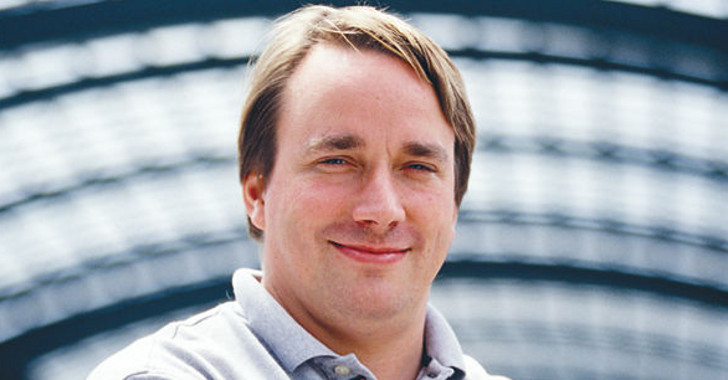
\includegraphics[width=0.4\textwidth]{images/Linus-Torvalds.jpg}}
      vs
    \fbox{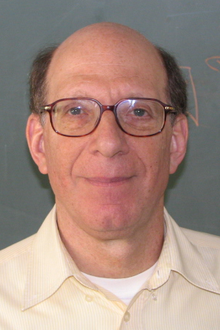
\includegraphics[width=0.2\textwidth]{images/Andrew-Tanenbaum.png}}
   \end{center}
\begin{center}
 	http://en.wikipedia.org/wiki/Tanenbaum%E2%80%93Torvalds_debate
\end{center}
\end{frame}

%%% Local Variables: 
%%% mode: latex
%%% TeX-master: "main"
%%% End:
